% !TEX root =../main.tex

\chapter{Vergleich bestehender Webshops}

In diesem Kapitel sollen populäre Webshops verglichen und im Bezug auf Social Commerce bewertet werden. Für die Bewertung werden die in Kapitel \ref{auswahl-konzepte} erarbeiteten Konzepte verwendet.


\section{Vergleich der Nutzer-Community}

Üblicherweise bietet die Nutzer-Community Hilfe und Tipps von Nutzern für Nutzer und bindet die Nutzer an bestimmte Richtlinien, um alle Mitglieder der Community zu schützen und fair zu behandeln. Das laut Meinung der Autorin primäre und wichtigste Kriterium ist hierbei, die Möglichkeit Tipps und Feedback zu geben. Online Hilfe und Richtlinien spielen laut Meinung der Autorin eine untergeordnete Rolle. Tabelle \vref{tab:tabelle-gruen} zeigt die Gegenüberstellung der ausgewählten Webshops.

\begin{table}[htbp]
	\centering
	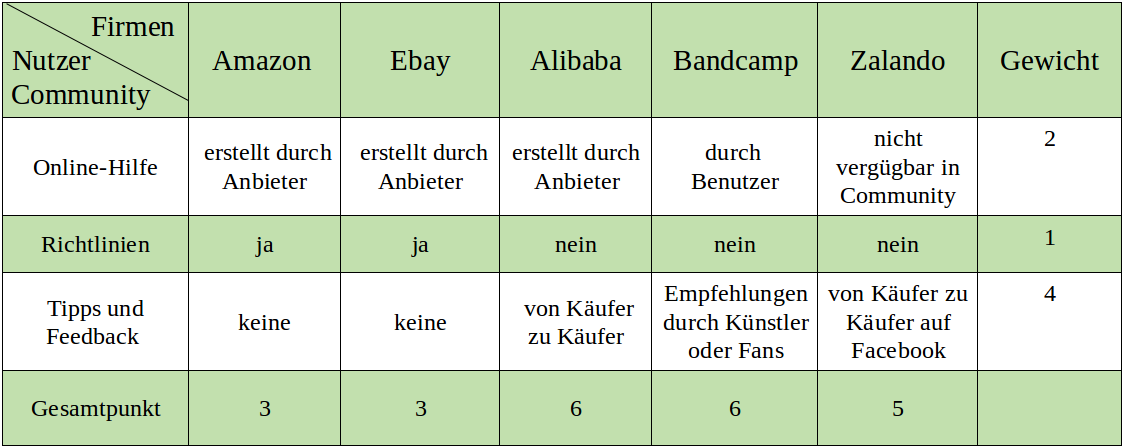
\includegraphics[width=1\textwidth]{bilder/tabelle-gruen.png}
	\caption{Nutzer-Community}
	\label{tab:tabelle-gruen}
\end{table}

In der Hinsicht bieten Alibaba und Bandcamp eine gute Plattform, sodass Nutzer miteinander kommunizieren können. Bei Alibaba geschieht dies durch ein separates Forum\footnote{Alibaba Community: \url{https://buyer.alibaba.com/forum}}. Bei Bandcamp\footnote{ Bandcamp Community: \url{https://bandcamp.com}} kann man sich nicht nur mit den Künstler verbinden, sondern auch mit anderen Fans Erfahrungen teilen.

Amazon\footnote{Amazon Community: \url{https://www.amazon.de/gp/help/customer/display.html?nodeId=201483620}} und Ebay\footnote{Ebay Community: \url{https://pages.ebay.de/help/policies/member-created-content-ov.html\#policy}} bieten auch Communities an. Deren Funktionen orientieren sich an der Online-Hilfe und Richtlinien. Es ist keine direkte Benutzerinteraktion verfügbar. Ein Ausnahme ist Zalando, die Firma betreibt ihre Community direkt auf Facebook\footnote{Zalando Community: \url{https://de-de.facebook.com/pg/Zalando.co.uk/community/}}.

\begin{figure}[htbp]
	\centering
	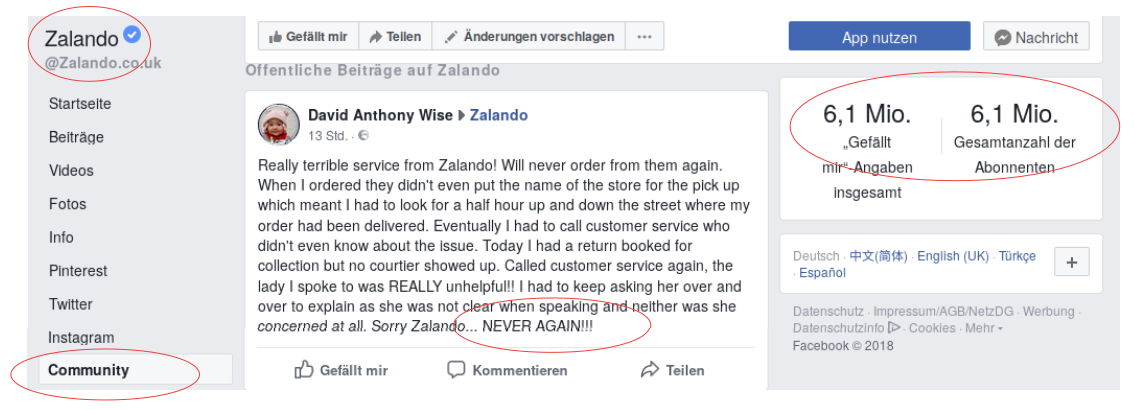
\includegraphics[width=1\textwidth]{bilder/zalando-community.png}
	\caption{Zalando Community auf Facebook}
	\label{fig:zalando-community}
\end{figure}

Wie in Abbildung \vref{fig:zalando-community} zu sehen, hat diese Maßnahme auch einige Nachteile. Z. B. muss man mit den Richtlinien von Facebook koexistieren. Zalando kann nicht die Kommentare kontrollieren. Ein weiter Nachteil ist, dass die schwerer für den Nutzer zu finden ist.


\section{Vergleich der Online-Kommunikation}

Um die online Kommunikation von Webshops zu bewerten, wurden durch die Autorin die Kriterien Real-Time Chatten, Fotos senden und verfügbare Sprachkanäle ausgewählt. Das laut Meinung der Autorin primäre und wichtigste Kriterium ist hierbei, die Möglichkeit zum Real-Time Chatten. Fotos senden und zusätzliche Sprachkanäle spielen laut Meinung der Autorin eine untergeordnete Rolle.

Online Kommunikation (Real-Time Chatten) spielt für Webshops eine immer größere Rolle. Die Statistik von \textcite{aliyun}\footnote{Tochterfirma der Alibaba} zeigt, bis 12.2016 verwenden 100 Millionen Nutzer Aliwangwang. Dies ist eine spezielle Software für Real-Time Chatten und wird Hilfswerkzeug von Alibaba eingesetzt. Amazon unterstützt offensichtlich nicht diese Funktion. Zalando hat hierbei das gleiche Problem wie Amazon. Auf der Webseite von Zalando steht ebenfalls keine Echtzeit-Kommunikation zur Verfügung. \parencite{piatscheck}

Tabelle \vref{tab:tabelle-grau} stellt die Online Kommunikation der ausgewählten Webshops gegenüber.

\begin{table}[htbp]
	\centering
	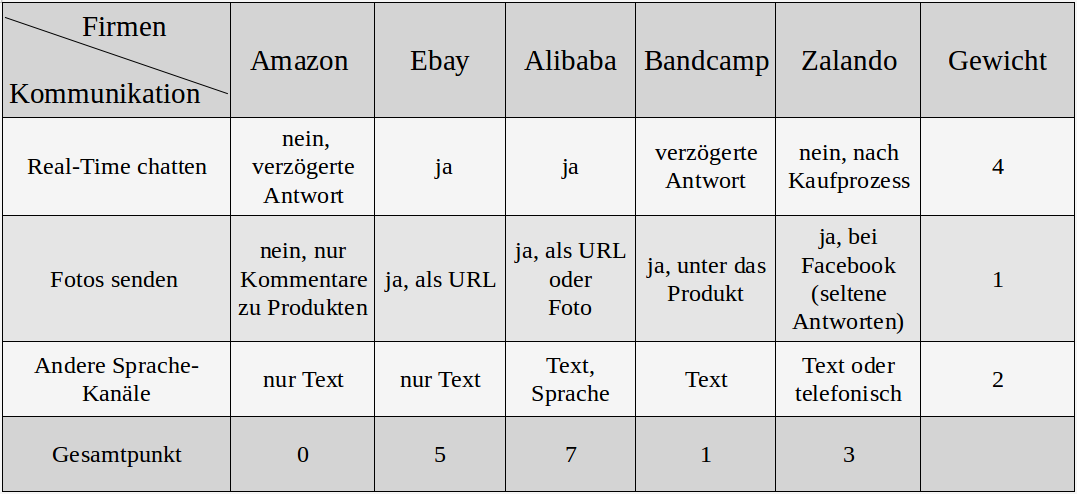
\includegraphics[width=1\textwidth]{bilder/tabelle-grau.png}
	\caption{Online Kommunikation}
	\label{tab:tabelle-grau}
\end{table}


\section{Vergleich der Produktvielfalt}

Nach der Statistik von \textcite{statista} wird bestätigt, dass der Gewinn abhängig von der Vielfalt der angebotenen Produkten ist. Nach der Meinung von Richard Lazazzera, How to Choose an Ecommerce Business Model\footnote{\url{https://www.shopify.com/blog/17240328-how-to-choose-an-ecommerce-business-model}} werden Businessmodelle unterschiedliche Kriterien unterteilt. Davon ist die Beziehung zwischen Käufer und Verkäufer die wichtigste. Danach belegen Marktpositionierung und Spezialisierung auf einen Produktbereich den zweiten Platz.

Tabelle \vref{tab:tabelle-rot} stellt die Geschäftsmodelle, Verkaufsmodelle und Produktarten der ausgewählten Webshops gegenüber.

\begin{table}[htbp]
	\centering
	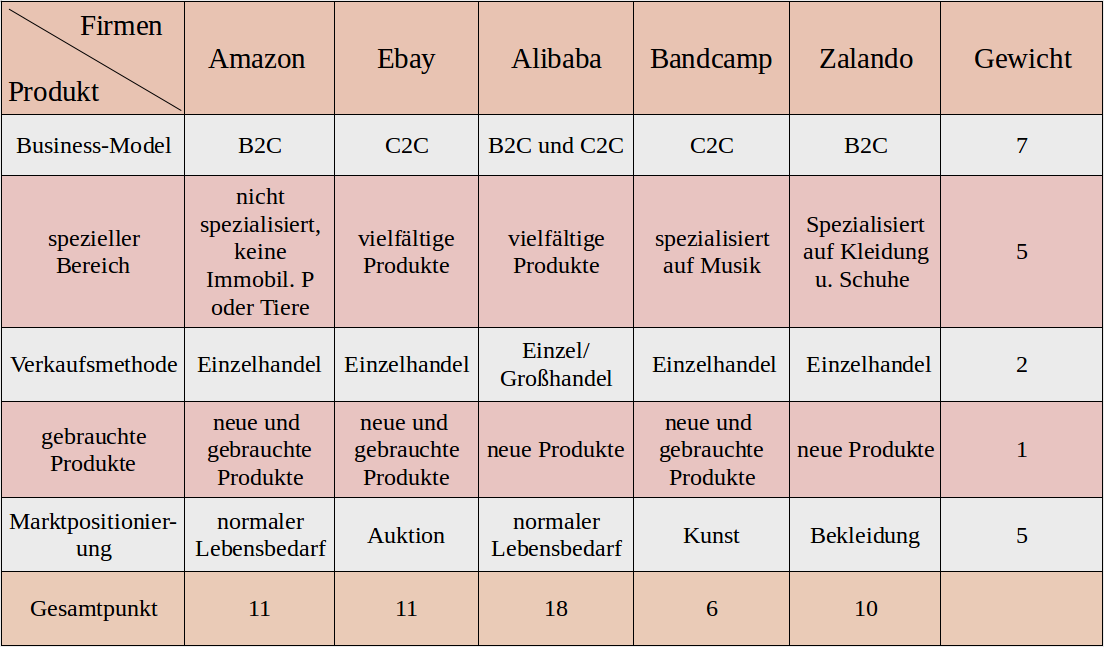
\includegraphics[width=1\textwidth]{bilder/tabelle-rot.png}
	\caption{Produktvielfalt}
	\label{tab:tabelle-rot}
\end{table}


\section{Vergleich der Zahlungsmethoden}

Weil Alibaba eine eigne Zahlungsmethode besitzt (Alipay - www.alipay.com), kann der Handelsbereich von Alibaba in den Finanzsektor erweitert werden. Unter der Prämisse die Sicherheit von Zahlungsinformation nicht zu verletzen haben Nutzer mehrere Möglichkeiten zu bezahlen. Andere Online Shops verwenden hierbei noch die Finanzprodukte von anderen Unternehmen, z.B. von Banken, PayPal usw. .

Um die Zahlungsmethoden von Webshops zu bewerten, wurden durch die Autorin die Zahlungsmöglichkeiten Kreditkarte, Giro-Karte, online Bezahldienste und eigne Finanzservices ausgewählt. Das laut Meinung der Autorin primäre und wichtigste Kriterium ist hierbei, die Möglichkeit \term{pay by others} zu nutzen. Bei den eigenen Finanzservices kann das Finanzprodukt durch den Provider selbst skaliert und gestaltet werden. Diese spielen aus diesem Grund laut Meinung der Autorin auch eine schwerwiegende Rolle.

Tabelle \vref{tab:tabelle-rot} stellt die Zahlungsmethoden der ausgewählten Webshops gegenüber.

\begin{table}[htbp]
	\centering
	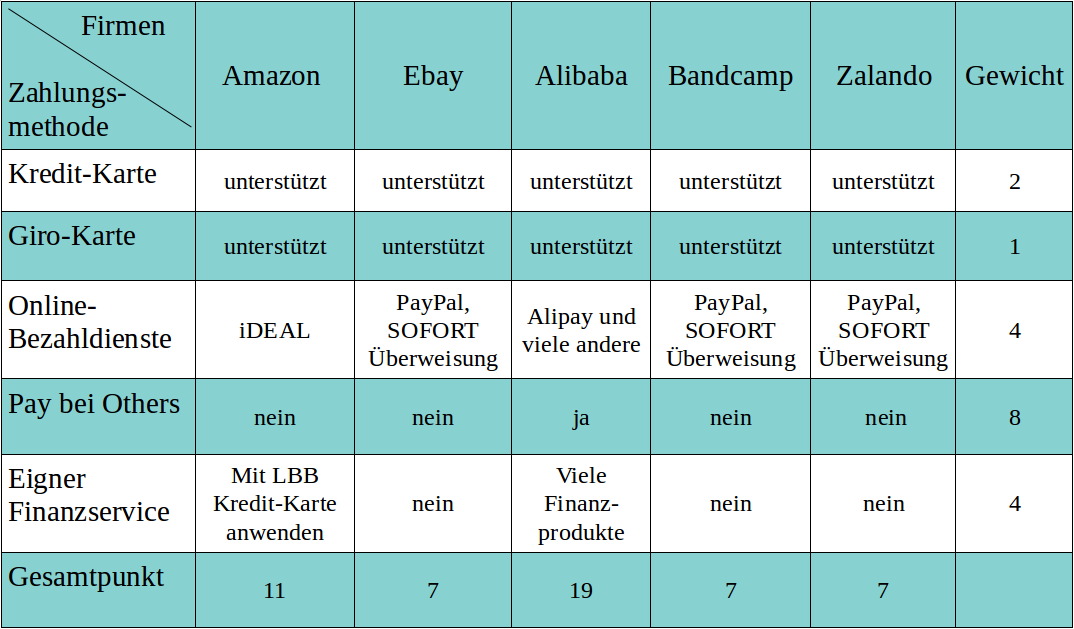
\includegraphics[width=1\textwidth]{bilder/tabelle-blau.png}
	\caption{Zahlungsmethoden}
	\label{tab:tabelle-blau}
\end{table}


\section{Vergleich der Methoden der Bewertung}

Bei der Bewertung bieten Amazon und Alibaba unterschiedliche Vorgehensweisen zum kommentieren an. So ist z. B. die Bewertung bei Amazon in Form von Sternen und einem Kommentar-Text realisiert. 1 bis 5 Sterne zeigen hier das Level der Zufriedenheit von unzufrieden bis sehr zufrieden. Abbildung \vref{fig:bewertung-amazon} zeigt Bewertungen in Amazon.

\begin{figure}[htbp]
	\centering
	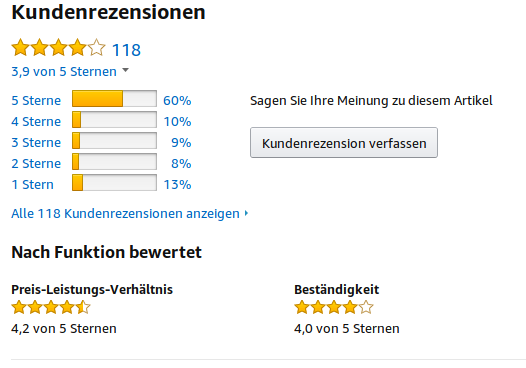
\includegraphics[width=1\textwidth]{bilder/bewertung-amazon.png}
	\caption{Bewertungen in Amazon}
	\label{fig:bewertung-amazon}
\end{figure}

Die rege Nutzung der Kommentare unter Produkten zeigt, immer mehrere Kunden wollen eine Bewertung abgeben, damit andere Nutzer Tipps oder Hinweise erhalten können. Die Webshops erstellen hierfür unterschiedliche Methoden, sodass die Bewertung konkreter und intuitiver sind. Nach der Meinung der Autorin sind diese zusätzlichen Methode für die Nutzer wichtig und nötig.

Tabelle \vref{tab:tabelle-gelb} stellt die Methoden der Bewertung für die ausgewählten Webshops gegenüber.

\begin{table}[htbp]
	\centering
	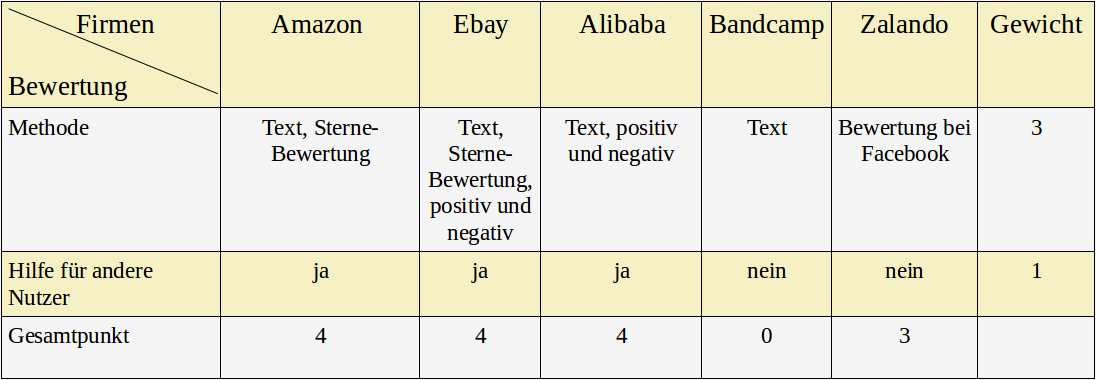
\includegraphics[width=1\textwidth]{bilder/tabelle-gelb.png}
	\caption{Methoden der Bewertung}
	\label{tab:tabelle-gelb}
\end{table}

\newpage


\section{Gesamtergebnis}

Tabelle \vref{tab:tabelle-ergebnis} stellt das Gesamtergebnis der ausgewählten Webshops gegenüber.

\begin{table}[htbp]
	\centering
	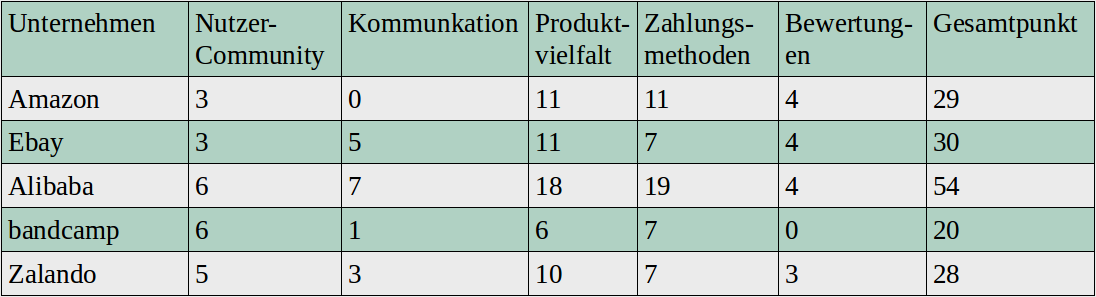
\includegraphics[width=1\textwidth]{bilder/tabelle-ergebnis.png}
	\caption{Gesamtergebnis}
	\label{tab:tabelle-ergebnis}
\end{table}

Nach der Berechnung des Gesamtergebnis können wir durch ein Diagramm zeigen, welcher Anbieter dominant ist. Abbildung \vref{fig:diagramm-ergebnis} stellt das Gesamtergebnis dar.

\begin{figure}[htbp]
	\centering
	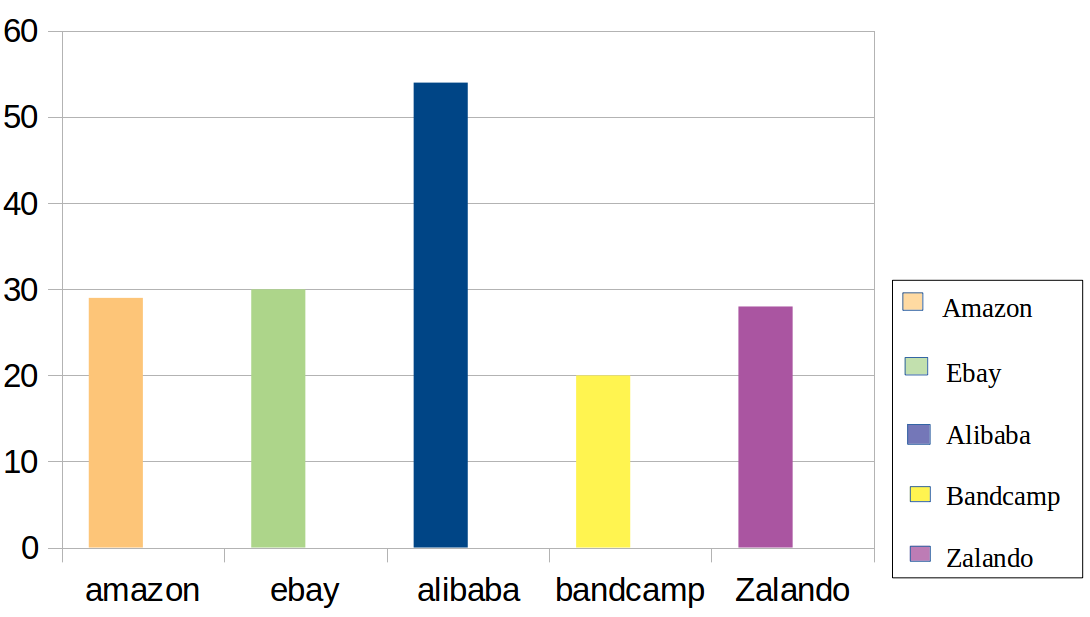
\includegraphics[width=0.7\textwidth]{bilder/diagramm-ergebnis.png}
	\caption{Auswertung Gesamtergebnis}
	\label{fig:diagramm-ergebnis}
\end{figure}

Das Diagramm zeigt als Ergebnis, dass im Vergleich zu anderen Firmen Alibaba die höchste Anzahl an Punkten erlangt hat. Der in dieser Arbeit zu konzipierende Shop soll die Vorteile von Alibaba aufgreifen und so die Servicequalität als Webshop weiter erhöhen.


\section{Auswertung} 

In den vorigen Abschnitten verglich die Autorin die Dienstleistungen, die von fünf Webshops in denen Benutzer-Communities, Echtzeitkommunikation, Zahlungsmethoden und Produktbewertungen angeboten werden. Unter ihnen belegte Alibaba mit 54 Punkten den ersten Platz, gefolgt von Amazon und Ebay auf den Plätzen zwei und drei. Bandcamp und Zalando erzielen die niedrigste Punktzahl.

Im Vergleich dazu können wir sehen, dass die drei besten Ergebnisse diejenigen mit der größten Anzahl an Kunden und bei den Nutzern sehr beliebt sind. Unter ihnen bietet Alibaba eine größere Anzahl an Mehrwertdiensten als andere Unternehmen.

Mehrwertdienste sind sehr wichtig für die Entwicklung des Unternehmens: Der Webshop ist nicht länger nur ein Geschäft. Seine Gewinnquellen sind tendenziell diversifiziert. Zum Beispiel, in Bezug auf Zahlungsmethoden, haben Amazon und Alibaba ihre eigenen Finanzderivate entwickelt. Amazon und Banken kooperieren, um Kredit-Homeshopping anzubieten, so dass Benutzer komfortabel bezahlen können. Alibaba hat ein eigenes Zahlungssystem entwickelt, um \glqq{}Bargeldlose\grqq{} Zahlungen zu ermöglichen. Bei Alipay ist darüber hinaus ist zu beachten, dass die Zins- und Kapitalerträge, die durch die riesige Währungseinlage generiert werden, nicht unterschätzt werden sollten.

Die Nutzergemeinschaft, die Produkte und die Evaluierungsservices sorgen für ein besseres Einkaufserlebnis für die Nutzer, sodass diese länger im Webshop bleiben wollen. Der Fachbegriff Customer Stickiness wird verwendet, um zu beschreiben, dass eine erfolgreiche Website die Nutzer dazu motiviert, viel Zeit auf einer Plattform zu verbringen und somit in Webshops einen kontinuierlichen Verkauf und Ausbau zu erreichen. Je höher die Customer Stickiness, desto beliebter ist die Website und desto höher ist ihr Geschäftswert. Ein typisches Beispiel hierfür ist YouTube. Anzeigen werden eher auf Websites platziert, die bei Nutzern beliebt sind und auf denen Nutzer für längere Zeit verweilen.

Customer Stickness ist somit von großer Bedeutung. Laut \textcite{bradlow-wharton} Professor der Wharton University of Pensylvania ist sie wie folgt definiert: \glqq{}Customer stickiness is the increased chance to utilize the same product or service that was bought in the last time period. Due to Levi’s customer stickiness for its jeans, people who try Levi’s, buy pairs over and over again.\grqq{}

Webseiten mit geringer Customer Stickiness zeigen sich darin, dass sich der Benutzer versehentlich durch die Suche nach einem Produkt an sie erinnert und sich anmeldet. Nachdem die Nutzung abgeschlossen ist, verlässt der Benutzer umgehend die Webseite. Der bereitgestellte Dienst wird normalisiert und die \glqq{}überzählige\grqq{} Erfahrung des Benutzers ist nicht zufriedenstellend.\\
\parencite{localytics}

Der kooperativen Webshop, der durch die Autorin konzipiert werden soll, zielt daher auch darauf ab, mehr Benutzer anzuziehen, mehr Dienste und Funktionen bereitzustellen, das erwartete Einkaufserlebnis des Benutzers zu befriedigen und die Customer Stickiness des Benutzers zu verbessern.

Der zu konzipierende Webshop soll die Vorteile beliebter Webshops vereinen und hat mehr Funktionalität bieten, die nicht nur die Mängel anderer Websites ausgleichen, sondern auch die Interaktion zwischen den Nutzern erheblich erhöhen, was das Einkaufen komfortabler und interessanter macht.

% TODO: Kann das nachfolgende gelöscht werden?

%\section{Notizen}

%Eher Social E-Commerce oder?

%Der Begriff Social Commerce wurde dem gleichnamigen Buch \parencite{turban:sc} entnommen. Den Begriff würde ich nur ungern abwandeln. 

%Welche [Geschäftsmodelle] gibt es in der Richtung überhaupt? Kläre mich auf. 

%\begin{itemize}
%\item Free (z. B. Facebook)
%\item Freemium (z. B. Spotify, XING, GitHub)
%\item Long Tail – Angebot von Nischenprodukten (z. B. Itunes)
%\item Marktplatzmodell (z. B. Amazon, Ebay)
%\end{itemize}

%Es gibt unterschiedliche Geschäftsmodelle, für meine Arbeit werden Marktplatzmodell benutzen, die Plattform für die Käufer kostenlos, für die Verkäufer wird Freemium angewendet.

%Wie könnte dieses Konzept aussehen? 

%Konzept würde aus folgenden Teilen bestehen: 
%\begin{itemize}
%\item Geschäftsmodell 
%\item Oberflächendesign 
%\item Funktionaltät/Features 
%\item Umsetzung von Anwendungsfällen beschreiben 
%\end{itemize}

%Welche Kommunikationskanäle sollen genutzt werden? 

%Zwischen Kunden

%\begin{itemize}
%\item Text (Instant Messenging) 
%\item Sprache 
%\item Video 
%\item Bewertungen 
%\end{itemize}

%Zwischen Kunde und verkäufer 

%\begin{itemize}
%\item Text 
%\item Sprache 
%\item Bewertungen 
%\end{itemize}

%Welche Methode nutzt du zur Untersuchung? Wie soll diese Erfolgen?

%\begin{itemize}
%\item Case-based Evidence als Methode zur Untersuchung 
%\item Auf Basis von Anforderungen wird überprüft, ob eine bereits existierende Software diese Anforderung erfüllt 
%\item Beispielsweise könnte eine Anforderung sein, dass der Nutzer seinen Avatar in einer 3D-Umgebung bewegen und steuern muss 
%\item Computer spiele haben genau diese Anforderung bereits erfolgreich erfüllt 
%\end{itemize}

%Was ist deine Hypothese bzw. welches Ergebnis erwartest du?

%\begin{itemize}
%\item Durch die Verbindung von E-Commerce, Social Media und Computerspielen kann kooperatives Einkaufen ermöglicht werden 
%\item Kooperatives Einkaufen eignet sich besonders für subjektive Kaufentscheidungen 
%\item Shops liefern bisher eher Hilfe bei objektiven Kaufentscheidungen (Testberichte und Bewertungen fremder Nutzer) 
%\item Für subjektive Einschätzungen ist vor allem die Meinung von Freunden wichtig 
%\end{itemize}

%Welche Anwendungsfälle – die musst du schon hier darlegen.

%\begin{itemize}
%\item Zwei Personen verabreden sich zum gemeinsamen Einkaufen 
%\item Während des Einkaufens benötigt eine Person Hilfe bei einer Kaufentscheidung und lädt einen Freund ein ihr zu helfen 
%\item Kunde kann mit Verkäufer kooperativ interagieren 
%\item Kunde kann Geld zu anderem Kunden transferieren
%\end{itemize}
